\documentclass[twoside,11pt]{article}

\usepackage{jmlr2e}
\usepackage{spverbatim}
\usepackage{amsmath}

\begin{document}

\title{Learning with Nearest Neighbor}

\author{\name Andrew Kirby \email andy-kirby@live.com \AND
		\name Kevin Browder \email browderkevin54@gmail.com \AND
		\name Nathan Stouffer \email nathanstouffer1999@gmail.com \AND
		\name Eric Kempf \email erickempf123@gmail.com }

\maketitle

\begin{abstract}
	K-Nearest Neighbors is a non-parametric learning method that may be used for classification or regression. This learning model is versatile and may be used in situations where the distribution is known or unknown. Through tuning and experimentation, the K-Nearest Neighbors algorithm and several variants that help reduce the amount of data needed by the learner are explored, revealing their strengths and pitfalls.

\end{abstract}

\section{Problem Statement}

In the realm of machine learning, knowing the form of some distribution of data is valuable information. In these cases, parametric learning may be used, mimicking the distribution with a fixed set of parameters and forms. An example of this is Naive Bayes, which can be learned quickly and represented simply. These learning algorithms train fast and require relatively less data. The limitation of parametric learning is that the functional form of the algorithm constrains the performance \citep{distance-k-nn}.

The data sets to be handled in this project do not follow a known distribution \citep{datasets}. Thus, constructing parametric learners for these sets is difficult. Non-parametric learning offers a solution to this problem, making no strong assumptions about the form of the data---and therefore not constructing a model with a fixed form.

One popular and intuitive method of non-parametric learning is the K-Nearest Neighbors (K-NN) learning algorithm \citep{NNClassificationOrigPaper}. Given data sets containing examples, the task is to implement K-NN learning algorithm for both classification and regression problems. Given the same input file, a secondary task is to reduce the size of the data set by implementing the Edited Nearest Neighbor (E-NN), Condensed Nearest Neighbor (C-NN), K-Means (KMeans), and K-Medoids (PAM) data reducing algorithms. Of particular are interest is how the data reducers contribute to the performance of K-Nearest Neighbor.

\subsection*{Hypothesis}

K-NN is expected to outperform the other nearest neighbor variants. K-NN utilizes the most data points from the data set, which is essential for minimizing the error rate. Furthermore, KMeans and PAM are expected to perform better than E-NN and C-NN because they will have similar amounts of representative points, but KMeans and PAM fit the representative points to the known data.

\section{Algorithms}

\subsection{K-NN}

K Nearest Neighbor (K-NN) is a modification of the nearest neighbor rule, a nonparametric procedure for classification or regression that utilizes a set of known points.

At its core, the nearest neighbor rule utilizes the intuitive assumption that a set of known examples, $X$, follows the distribution of all possible examples that it was taken from. As such, examples which are ``close" to each other likely belong to the same class or have a similar real value (\cite{NNClassificationOrigPaper}). Metrics for determining this distance are discussed in section 2.2.

Thus, given $X$, a number of neighbors $k$, and a query example $x$, K-NN finds the $k$ nearest neighbors of $x$ by iterating through the examples in $X$, calculating the distance from $x$ for each example. Then K-NN classifies $x$ given a majority vote among the returned class values from its $k$ nearest neighbors. K-NN handles regression by computing the mean value among its $k$ nearest neighbors.

Note that this does not heavily assume anything about the form of the actual distribution. K-NN is flexible enough to adapt to almost any functional form that the underlying distribution takes on. This is an advantage for data sets that are hard to visualize or have unknown traits. The downside to this characteristic is that, like many nonparametric models, K-NN requires much more data than a parametric model to effectively train. In other words, K-NN requires a great number of known examples because it is essentially estimating the real distribution from the known examples. Without sufficient data, K-NN will perform poorly.

In fact, the error of K-NN, $R_{knn}$ as the number of points sampled approaches infinity is bounded by:
$$R^* \leq R_{knn} \leq (1+\frac{1}{k})R^*$$
where $R^*$ is the Bayes risk, the optimal risk given a known set of probability densities that represents the data. Thus, as $k \rightarrow \infty$ and the number of data points $n \rightarrow \infty$, theoretically $R_{knn} \rightarrow R^*$. Of course, $\frac{k}{n} \rightarrow 0$ should be ensured so that $k$ is still only a small subset of the total data points $n$  (\cite{NNClassificationOrigPaper}). In short, K-NN will work optimally as the number of points sampled approaches infinity. As more attributes or data complexity is added, K-NN will approach its optimal condition slower given increasing $n$.


\subsection{Distance Metrics}

The nearest neighbor rule, and therefore K-NN, requires a distance metric to determine the theoretical ``distance" between two examples. A common distance metric---and the one used in this paper---is Euclidean distance. The Euclidean distance $D$ between two examples $x_1$ and $x_2$ is computed as:
$$D = \sqrt{\sum_{i=0}^{d}(a_1^i - a_2^i)^2}$$
where $d$ is the number of attributes the examples have, $a_1^i$ is the $i$-th attribute of $x_1$, and $a_2^i$ is the $i$-th attribute of $x_2$.

A Euclidean distance metric assumes that all data in a dataset is continuous. However, in the world of data science and this project, some attributes contain categorical values. One method to compute this distance is the Value Difference Metric (VDM). Note that the VDM relies on classification to compute a distance, so continuous regression values must be discretized by some method.

To compute a distance between two categorical values $x_1, x_2$ within one attribute $a$ using the VDM, find the following for each value:
$$ v_n = \sum _{i = 1}^{k} | \dfrac{N_{1i}}{N_1} - \dfrac{N_{2i}}{N_2} | $$
where $N_{1i}, N_{2i}$ are the number of examples in $a$ that are of the $i^{th}$ class and have values $x_1, x_2$ respectively, and $N_1, N_2$ are the number of examples in $a$ that are of the $i^{th}$ class.

Then compute the difference
$v_2 - v_1$.
This difference is considered to be the distance $v$ between the two categorical values $x_1$ and $x_2$ \citep{vdm}. The squared difference can now be included in the summation when computing Euclidean distance.

\subsection{Data Reducers}
The K-Nearest Neighbor decision rule is a lazy algorithm where the performance is a function of the number of training examples. Therefore, in terms of a learner's computational efficiency, the most favorable training set is the smallest set.
This is subject to the constraint that the model's performance is not compromised.

Thus, the optimal training set for a K-NN learner is the smallest set that is able to correctly identify the value of any query example.
The purpose of the following four algorithms is to reduce the size of the dataset without compromising the learner's performance. Since K-NN is lazy by nature, this will improve the computation time of the learner at query time.
% should I talk about not decreasing performance? That is what we are testing right


\subsubsection{Edited K-NN}
The discussion of algorithms that reduce the size of a training set begins with Edited K-Nearest Neighbor. Edited K-NN begins by training a K-NN learner $L$ with each example in an initial dataset $D^0$. Note that since multiple steps in the following algorithm rely on knowing the classification of $e$, Edited K-NN can only be used on classification problems.

The learner $L$ then classifies each example $e^0 \in D^0$. That is, for each example $e^0$, the learner $L$ returns the predicted class of $e^0$: $predclass(e^0)$. However, recall that $e^0$ is a training example, so $class(e^0)$, the actual class of $e^0$, is known. So, for each $e^0$ where $class(e^0) \neq predclass(e^0)$ (if $e^0$ was misclassified), the algorithm removes $e^0$ from $D^0$.

This creates a new set $D^1$. The learner $L$ is now trained with $D^1$ and the editing process repeats itself until performance decreases \citep{edited}. In this case, the performance is measured as the accuracy of the learner on a validation set. The validation set is consistent throughout all editing iterations.

Say performance decreases on the $i^{th}$ iteration. The final edited data set is $D^{i-1}$. A separate K-NN classifier is now trained using $D^{i-1}$ and subsequently tested.
% remember to discuss lack of knowledge about overfitting in convergence based algorithms

\subsubsection{Condensed K-NN}

The condensing reduces neighboring, similarly classed points into a single point.

Condensing begins with a null set $Z$ and initializes a random starting point in the data set. When the algorithm terminates, $Z$ will be the reduced data set. The algorithm iterates through all examples $x$ in the original data set and finds the closest example $x’$ in $Z$ for each of them. It then compares the classes of $x$ and $x’$, adding $x$ to the data set $Z$ only if the two classes differ. This process is repeated until $Z$ no longer changes, or the max number of iterations is reached.

This process can be thought of as simply taking all of the same class examples nearest each other and condensing them into a single point. This way, the number of points required to represent a class at any given point is reduced (\cite{Condensed}).

\subsubsection{Kmeans K-NN}

The K-Means algorithm utilizes clustering to return a smaller data set. This is performed by taking the average value of all the points in a cluster, and then re clustering and repeating until the averages converge.

The algorithm is passed in a data set and a value for number of clusters $K$. It then initializes $K$ clusters by randomly selecting points out of the data set. We chose to take the initial points from the data set in an effort to reduce the time it takes for the algorithm to zero in on the data. From there, the algorithm iterates through all of the examples in the original set and adds them to the nearest cluster. Once all points have been assigned, K-Means computes the new average point within each cluster and assigns that to the representative point. Once every cluster average has been recomputed, all points are reclustered based on the new representative points. This process is repeated until the representative points no longer change, or a max number of iterations is reached.

By recalculating the means of each cluster multiple times, the algorithm is predictable and the centroids will find their way to the same points, regardless of which points were first initialized (\cite{CMeans}).

\subsubsection{PAM K-NN}
The Partitioning Around Medoids (PAM) K-NN is a variant of K-Means K-NN but is more resistant to outliers because it uses an actual point in the data set instead of average the examples in a cluster. PAM begins by randomly selecting $C$ number of data points from the data set $D$ as the medoids $m$. In this case $C$ is determined by the number of points returned by Edited K-NN. The algorithm then clusters all of the remaining examples $x$ to the closest corresponding $m_i \in m$. Then the distortion is calculated with 
$$D = \sum_{j=1}^{k}\sum_{i \in cluster_j} (x_i - m_j)$$
where $x_i$ is the $i^{th}$ example in the $j^{th}$ cluster. Now iterate through each $m$ and swap it with every $x_j \in D$ such that $x_j \notin m$. After every swap the distortion $D$ is calculated again. This was optimized by calculating the distortion of each medoid separately and only recalculating the distortion for the medoid that was changed. If the new distortion is less than the original distortion the algorithm moves on and if the new distortion is greater than the original distortion than the medoid and example are swapped back. The clusters are then cleared and the algorithm then recalculates all of the clusters and distortion and repeats the swapping until no more swapping occurs or the algorithm iterates through 1000 times (\cite{Fox1990FindingGI}).

\section{Experiment}

\subsection{Preprocessing Choices}

First, all the examples in the data set are randomly scrambled and then assigned to sets for ten-fold cross validation. All categorical variables are converted to integers and the preprocessor also generates a similarity matrix for each categorical variable that is used for determining distances between categorical variables. All numerical variables are normalized between 0 and 1. The data sets did not contain any missing variables so preprocessing did not to handle that.

\subsection{Tuning}

One parameter to tune is $C$, the number of representative points that K-Means K-NN and K-Medoids K-NN have. The following tables show the Mean Standard Error for both clustering algorithms on a sample of the data sets tested with different numbers of clusters. There are two sections, one for regression data sets and the other for classification data sets.

% the table should go in this exact spot
\begin{table}[h]
	%\title{Selected results of varying the number of clusters}
	\begin{minipage}[b]{0.45\linewidth}\centering
		Forest Fires MSE
		\begin{tabular}{lllll}
			\cline{1-4}
			\#Clusters & 0.15N   & 0.25N   & 0.35N   &  \\ \cline{1-4}
			KMEANS     & 4235.6  & 4238.05 & 4236.91 &  \\
			KMEDOIDS   & 4235.95 & 4236.03 & 4247.17 &  \\
		\end{tabular}
	\end{minipage}
	\hspace{0.5cm}
	\begin{minipage}[b]{0.45\linewidth}
		Forest Fires ME
		\centering
		\begin{tabular}{llll}
			\cline{1-4}
			\#Clusters & 0.15N  & 0.25N  & 0.35N  \\ \cline{1-4}
			KMEANS     & -12.71 & -12.63 & -12.66 \\
			KMEDOIDS   & -12.68 & -12.7  & -12.54
		\end{tabular}
	\end{minipage}
	%%%%%%%%%%%%%%%%%%%%%%%%%%%%%%%%%%%%%%%%%%%%%%%%%%%%%%%%%%%
	\begin{minipage}[b]{0.45\linewidth}\centering
		Machine MSE
		\begin{tabular}{llll}
			\hline
			\#Clusters & 0.15N & 0.25N & 0.35N \\ \hline
			KMEANS     & 2.08  & 2.05  & 2.05  \\
			KMEDOIDS   & 2.06  & 2.05  & 2.07
		\end{tabular}
	\end{minipage}
	\hspace{0.5cm}
	\begin{minipage}[b]{0.45\linewidth}
		Machine ME
		\centering
		\begin{tabular}{llll}
			\cline{1-4}
			\#Clusters & 0.15N & 0.25N & 0.35N \\  \cline{1-4}
			KMEANS     & -0.5  & -0.51 & -0.51 \\
			KMEDOIDS   & -0.51 & -0.51 & -0.51
		\end{tabular}
	\end{minipage}
	%%%%%%%%%%%%%%%%%%%%%%%%%%%%%%%%%%%%%%%%%%%%%%%%%%%
	\begin{minipage}[b]{0.45\linewidth}\centering
		Car Accuracy
		\begin{tabular}{llll}
			\hline
			\#Clusters & -10\% & \#ENN   & +10\% \\ \hline
			KMEANS     & 22.22\%      & 22.22\% & 22.22\%      \\
			KMEDOIDS   & 90.68\%      & 92.82\% & 92.94\%
		\end{tabular}
	\end{minipage}
	\hspace{0.5cm}
	\begin{minipage}[b]{0.45\linewidth}
		Car MSE
		\centering
		\begin{tabular}{llll}
			\hline
			\#Clusters & -10\% & \#ENN  & +10\% \\ \hline
			KMEANS     & 8217.6       & 8217.6 & 8217.6       \\
			KMEDOIDS   & 37.75        & 11.55  & 10.55
		\end{tabular}
	\end{minipage}
	\caption{Selected results of varying the number of clusters}
\end{table}

Beginning with the regression data sets (Forest Fires and Machine), the initial number of clusters was set to $ 0.25 * N$ where $N$ is the number of points in the initial data set. Two other values were tested: $ 0.15 * N$ and $ 0.35 * N$.
For all data sets depicted above, the difference between each respective metric value when varying the cluster size was negligible.
Specifically, the largest difference in the MSE of Forest Fires is less than 15 while the initial value MSE was 4236.03, there is essentially no change.
Furthermore, the largest difference in ME for Forest Fires was 0.16 while the initial ME was -12.7, also virtually no change in the metric.

Thus varying the number of clusters within $10\%$ of $0.25 * N$ appears to have no affect on the performance of the learner on the regression data sets.

Now view the classification data set Car. The base value for the number of clusters in a classification set is the value returned by E-NN on that same data set. Call this value $E$. Two other tested values for the number of clusters are: $ 0.9 * E$ and $ 1.1 * E$.
For the car data set, the performance metrics for KMeans did not vary when changing the number of clusters. This is most likely because of outliers in the data set, since the performance metrics for KMedoids does change with the number of clusters and KMedoids is more resistant to outliers than KMeans.
Looking at the performance metrics for KMedoids, the best performing number of clusters was $1.1 * E$.

Another input must also be tuned: $K$, the number of nearest neighbors to compare with a query point. The value starts with $K = sqrt(N)$ where $N$ is the number of examples in the data set \citep{learning-k}. The two other values of $K$ tested were $0.9 * K$ and $1.1 * K$.
In viewing Table 2 (which can be found in the Results section), it can be seen that, for classification data sets, the learner, on average, performs better when considering the $0.9 * K$ than the other possible values for $K$.
For regression data sets, there is no significant change.

\section{Results}

Tests were run to evaluate performances of each algorithm based on varying $k$ as well as KMeans and PAM given varying numbers of clusters. The results for the varying $k$ tests are shown in table 1. The algorithms were evaluated using accuracy, mean square error (MSE), and mean error (ME).

For classification, MSE is a good indicator of how far off the predicted distribution is from the actual distribution. Accuracy indicates how well the algorithm is classifying examples on an individual basis.

Mean Error (ME) and MSE will be used to evaluate the regression problems. MSE takes the distance between real and predicted values and squares it. ME is computed similarly, but will not square the difference. MSE shows the existence of outliers because the value will increase a square. ME shows whether the learner is over or under estimating the values in the test set.

\newpage

% the table should go in this exact spot
\begin{table}[h]
	\title{Results of $k$ tests}
	\begin{minipage}[b]{0.45\linewidth}\centering
		Abalone Accuracy
		\begin{tabular}{llll}
			\hline
			K      & -10\%   & sqrt(N) & 10\%    \\ \hline
			K-NN   & 26.17\% & 26.10\% & 26.19\% \\
			E-NN   & 25.19\% & 25.38\% & 25.25\% \\
			C-NN   & 26.07\% & 25.95\% & 26\%    \\
			Kmeans & 0.02\%  & 0.02\%  & 0.02\%  \\
			PAM    & 0.02\%  & 0.02\%  & 0.02\%
		\end{tabular}
	\end{minipage}
	\hspace{0.5cm}\centering
	\begin{minipage}[b]{0.45\linewidth}
		Abalone MSE
		\centering
		\begin{tabular}{llll}
			\hline
			K      & -10\%   & sqrt(N) & 10\%    \\ \hline
			K-NN   & 202.39  & 218.05  & 231.09  \\
			E-NN   & 317.47  & 323     & 346     \\
			C-NN   & 177.06  & 195.23  & 202.61  \\
			Kmeans & 6893.59 & 6893.59 & 6893.59 \\
			PAM    & 6893.59 & 6893.59 & 6893.59
		\end{tabular}
	\end{minipage}
	%%%%%%%%%%%%%%%%%%%%%%%%%%%%%%%%%%%%%%%%%%%%%%%%%%%%%%%%%%%
	\begin{minipage}[b]{0.45\linewidth}\centering
		Cars Accuracy
		\begin{tabular}{llll}
			\hline
			K      & -10\%   & sqrt(N) & 10\%    \\ \hline
			K-NN   & 93.06\% & 93.29\% & 92.65\% \\
			E-NN   & 91.96\% & 92.09\% & 92.28\% \\
			C-NN   & 66.72\% & 62.15\% & 65.79\% \\
			Kmeans & 22.22\% & 22.22\% & 22.22\% \\
			PAM    & 92.48\% & 92.88\% & 92.13\%
		\end{tabular}
	\end{minipage}
	\hspace{0.5cm}\centering
	\begin{minipage}[b]{0.45\linewidth}
		Cars MSE
		\centering
		\begin{tabular}{llll}
			\hline
			K      & -10\%  & sqrt(N) & 10\%   \\ \hline
			K-NN   & 10.95  & 9.6     & 11.45  \\
			E-NN   & 13.67  & 12.83   & 13.83  \\
			C-NN   & 883.45 & 1324.4  & 998.25 \\
			Kmeans & 8217.6 & 8217.6  & 8217.6 \\
			PAM    & 13.75  & 11.3    & 16.85
		\end{tabular}
	\end{minipage}
	%%%%%%%%%%%%%%%%%%%%%%%%%%%%%%%%%%%%%%%%%%%%%%%%%%%
	\begin{minipage}[b]{0.45\linewidth}\centering
		Segmentation Accuracy
		\begin{tabular}{llll}
			\hline
			K      & -10\%   & sqrt(N) & 10\%    \\ \hline
			K-NN   & 83.33\% & 83.33\% & 81.90\% \\
			E-NN   & 84.13\% & 83.07\% & 81.48\% \\
			C-NN   & 54.76\% & 50\%    & 45.24\% \\
			Kmeans & 14.29\% & 14.29\% & 14.29\% \\
			PAM    & 80.48\% & 82.38\% & 79.52\%
		\end{tabular}
	\end{minipage}
	\hspace{0.5cm}
	\begin{minipage}[b]{0.45\linewidth}
		Segmentation MSE
		\centering
		\begin{tabular}{llll}
			\hline
			K      & -10\% & sqrt(N) & 10\%  \\ \hline
			K-NN   & 2.11  & 2.11    & 2.46  \\
			E-NN   & 2.19  & 2.67    & 2.92  \\
			C-NN   & 6.09  & 7.77    & 9.49  \\
			Kmeans & 56.37 & 56.37   & 56.37 \\
			PAM    & 2.57  & 2.14    & 2.86
		\end{tabular}
	\end{minipage}
	%%%%%%%%%%%%%%%%%%%%%%%%%%%%%%%%%%%%%%%%%%%%%%%%%%%
	\begin{minipage}[b]{0.45\linewidth}\centering
		Forest Fires MSE
		\begin{tabular}{llll}
			\hline
			K      & -10\%   & sqrt(N) & 10\%    \\ \hline
			K-NN   & 4239.7  & 4238.9  & 4238.22 \\
			Kmeans & 4235.71 & 4236.26 & 4238.24 \\
			PAM    & 4238.7  & 4248.17 & 4238.87
		\end{tabular}
	\end{minipage}
	\hspace{0.5cm}\centering
	\begin{minipage}[b]{0.45\linewidth}
		Forest Fires ME
		\centering
		\begin{tabular}{llll}
			\hline
			K      & -10\%  & sqrt(N) & 10\%   \\ \hline
			K-NN   & -12.64 & -12.65  & -12.67 \\
			Kmeans & -12.72 & -12.67  & -12.65 \\
			PAM    & -12.66 & -12.57  & -12.63
		\end{tabular}
	\end{minipage}
	%%%%%%%%%%%%%%%%%%%%%%%%%%%%%%%%%%%%%%%%%%%%%%%%%%%
	\begin{minipage}[b]{0.45\linewidth}\centering
		Machine MSE
		\begin{tabular}{llll}
			\hline
			K      & -10\% & sqrt(N) & 10\% \\ \hline
			K-NN   & 2.08  & 2.07    & 2.07 \\
			Kmeans & 2.07  & 2.06    & 2.06 \\
			PAM    & 2.07  & 2.07    & 2.06
		\end{tabular}
	\end{minipage}
	\hspace{0.5cm}\centering
	\begin{minipage}[b]{0.45\linewidth}
		Machine ME
		\centering
		\begin{tabular}{llll}
			\hline
			K      & -10\% & sqrt(N) & 10\%  \\ \hline
			K-NN   & -0.5  & -0.5    & -0.51 \\
			Kmeans & -0.51 & -0.51   & -0.51 \\
			PAM    & -0.51 & -0.51   & -0.51
		\end{tabular}
	\end{minipage}
	%%%%%%%%%%%%%%%%%%%%%%%%%%%%%%%%%%%%%%%%%%%%%%%%%%%
	\centering
	\begin{minipage}[b]{0.45\linewidth}\centering
		Wine Quality MSE
		\begin{tabular}{llll}
			\hline
			K      & -10\% & sqrt(N) & 10\%  \\ \hline
			K-NN   & 18.69 & 18.69   & 18.69 \\
			Kmeans & 18.69 & 18.69   & 18.69 \\
			PAM    & 18.69 & 18.69   & 18.69
		\end{tabular}
	\end{minipage}
	\hspace{0.5cm}\centering
	\centering
	\begin{minipage}[b]{0.45\linewidth}
		Wine Quality ME
		\centering
		\begin{tabular}{llll}
			\hline
			K      & -10\% & sqrt(N) & 10\%  \\ \hline
			K-NN   & -4.09 & -4.09   & -4.09 \\
			Kmeans & -4.09 & -4.09   & -4.09 \\
			PAM    & -4.09 & -4.09   & -4.09
		\end{tabular}
	\end{minipage}
	\caption{Results of varying $k$ for K-NN and variants. The middle $k$ value is the square root of $N$, the number of points in the set. Selected are $+/- 10\%$ of this number $N$.}
\end{table}

A standout may be the abysmal performance of K-NN and variants on the abalone data set. The K-NN learner's average accuracy is around 26\%. In the abalone dataset, the goal is to classify the age of an abalone mollusks. However, there are 29 ages and consecutive ages would be closely related to each other. Adjacent ages likely have attributes which blend together, making the problem particularly difficult for a nearest neighbor classifier whose weakness is this phenomena.
Additionally, 17 classes in the dataset have less than 100 examples associated with them \citep{datasets}, which is a small training set for a K-NN learner.
This makes creating a good model for the abalone dataset a difficult task.

One method to improve the accuracy of classification would be to bin the ages into three age categories and then use a K-NN learner to classify the examples in abalone. In one study, this resulted in accuracies as high as $56.67\%$ with a K-NN learner where $K = 1$ \citep{abalone-bad}.

% the graph should go in this exact spot
\begin{figure}[h]
	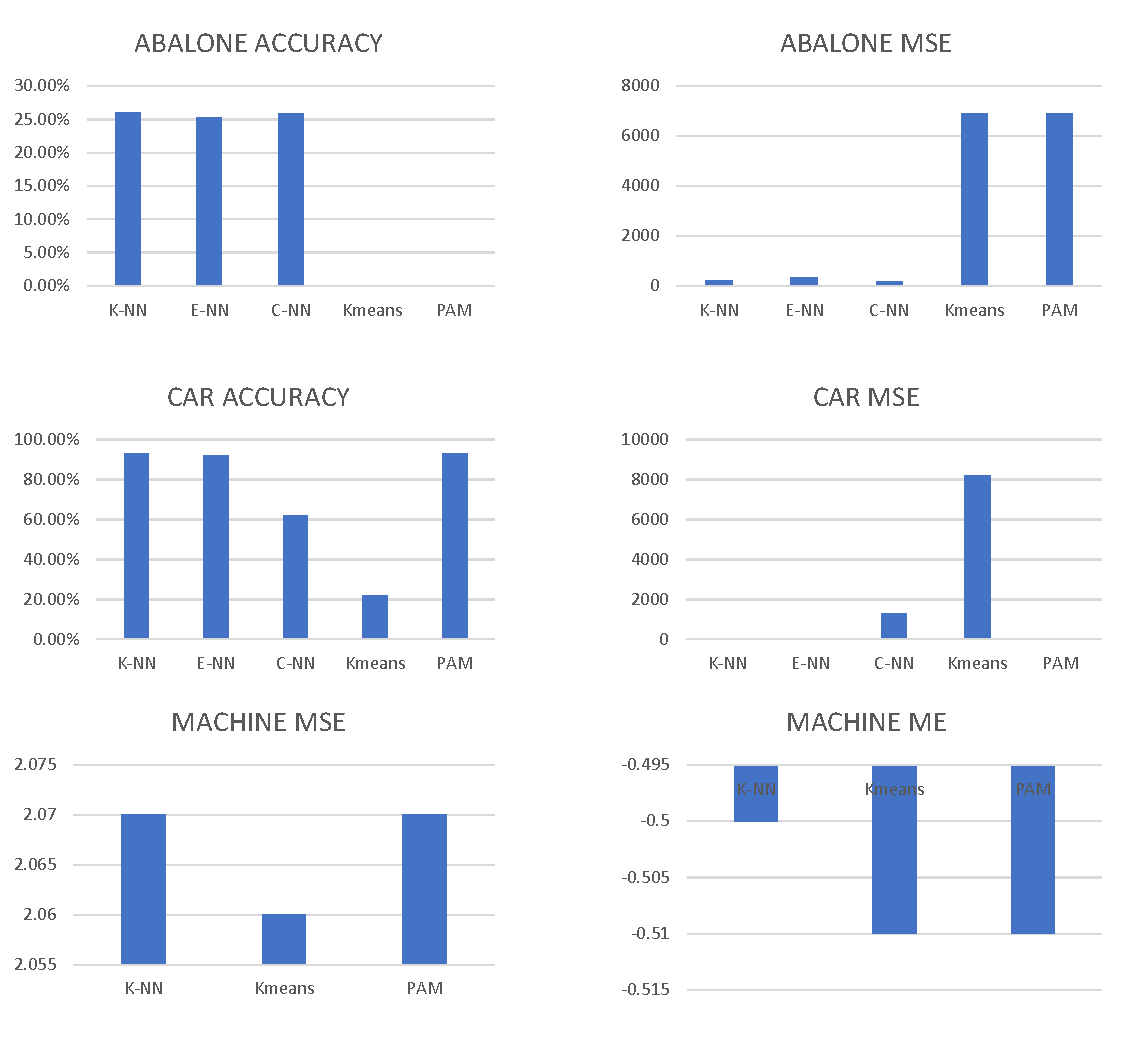
\includegraphics[width=\linewidth]{comparisongraphs.pdf}
	\caption{Graphical summary of each algorithm's performance on two classification sets and a regression set. Accuracy is computed with zero-one loss, MSE is the mean squared error, and ME is the mean error.}
	\label{fig:comparealgs}
\end{figure}

Selected comparisons of the tested algorithms are displayed in Figure 1. Of the K-NN variants used to reduce the number of data points needed, E-NN and C-NN generally trailed slightly behind K-NN, admittedly because they did not remove a large proportion of points from the original data set. PAM performed well in most data sets except for abalone, which most likely was not conducive to clustering. KMeans performed the worst out of the algorithms, likely due to its sensitivity to outliers. It was observed during implementation that the means would be pulled far from their clusters by outliers, leaving empty clusters when the clusters were repopulated. This highlights the advantages that PAM provides against KMeans.


\section{Summary}

K-NN offers the flexibility of nonparametric learning but is countered by the need to store large quantities of data. Thus, its variants that reduce the representative data set may be quite valuable when storage and computation time is critical. The user must be careful, however, to verify that these variants function properly and do not compromise performance. E-NN and C-NN fail to reduce the set effectively when the data distribution is overly complex. Kmeans is highly susceptible to outliers and PAM is computationally expensive when using optimal clusters. All nearest neighbor rule algorithms require very large data sets to achieve desired performance, especially as the data takes on more dimensions.


\bibliography{report}

\end{document}
